%%% Choose between 16:9 and 4:3 format by commenting out/uncommenting one of the following lines:
\documentclass[aspectratio=169]{beamer} % 16:9
% \documentclass{beamer} % 4:3

%=========================================================================================================================

\usepackage[english]{babel}     % English language
\usepackage[utf8]{inputenc}     % Input encoding changed to utf8 for proper rendering of umlauts
\usepackage{tikz}               % For creating graphics
\usepackage{subfig}
\usepackage[mode=buildnew]{standalone}
\usepackage{url}                % For including urls
\usepackage{tabularx}           % For better tables
\usepackage{xcolor}             % Für bunte Farbe :)

\usetheme{aig}                  % Set beamer theme

%=========================================================================================================================
\title{Qualität von Wikipedia-Artikeln}
\author[Kunze, Bunge, Krämer, Steenhof, Suxdorf]{Alexander Kunze, Sebastian Bunge, Johannes Krämer, Emmanuelle Steenhof, Robin Suxdorf}
\institute{Artificial Intelligence Group,\\
University of Hagen, Germany}
\date{\today}
%=========================================================================================================================
\logo{
\includegraphics[width=3cm]{figures/logoaig.png}}
%=========================================================================================================================

\begin{document}

%=========================================================================================================================

% frame
% block
% alertblock
% exampleblock

% \highlight{}
% \darkhighlight{}
% \yellowhighlight{}
% \mathhighlight{}
% \darkmathhighlight{}
% \yellowmathhighlight{}

% appendix

\begin{frame}
    \titlepage
\end{frame}
\nologo

\begin{frame}{Motivation}
    \begin{figure}
        \centering
        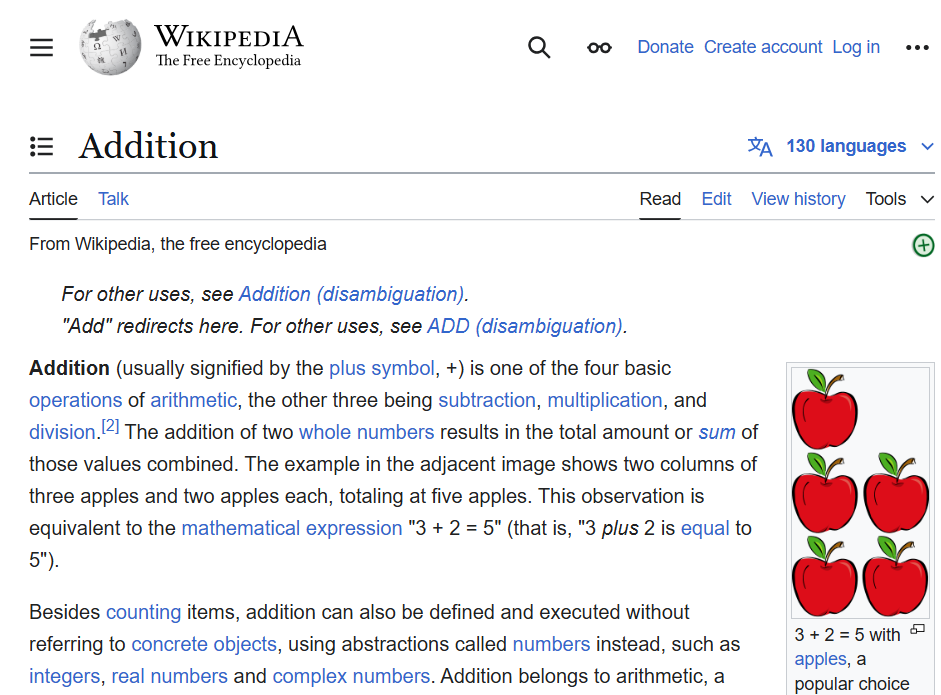
\includegraphics[width=0.6\linewidth]{figures/wp-screenshot-good.png}
        \caption{\url{https://en.wikipedia.org/wiki/Addition}}
    \end{figure}
\end{frame}

\begin{frame}{Motivation}
    \begin{figure}
        \centering
        
\includegraphics[width=0.6\linewidth]{figures/wp-screenshot-promo.png}
        \caption{\url{https://en.wikipedia.org/wiki/Brave_(web_browser)}}
    \end{figure}
\end{frame}

\begin{frame}{Motivation}
    \begin{figure}
        \centering
        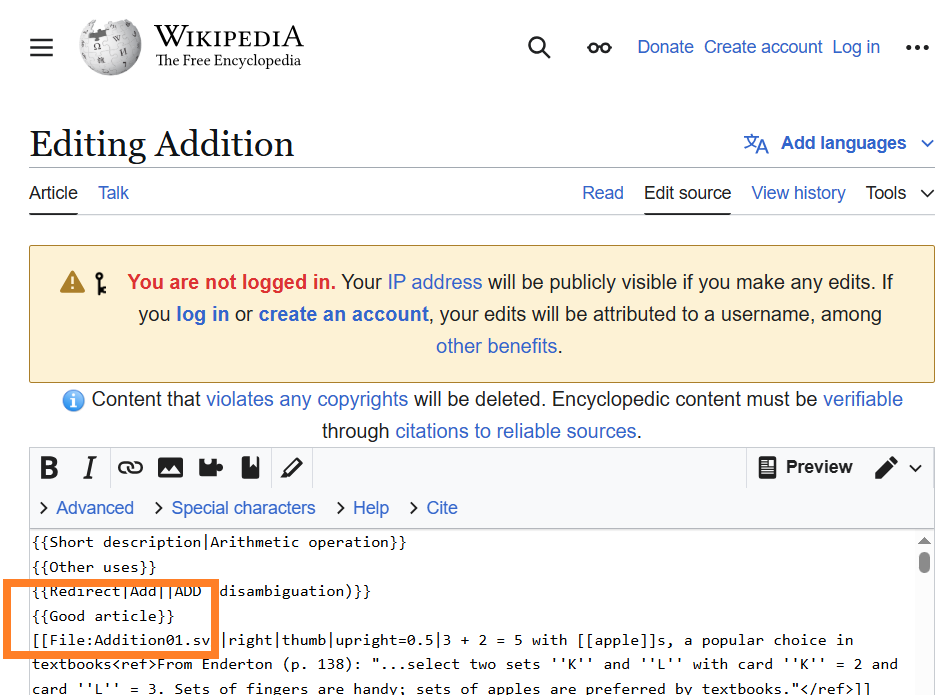
\includegraphics[width=0.6\linewidth]{figures/wp-screenshot-good-source.png}
        \caption{\url{https://en.wikipedia.org/w/index.php?title=Addition&action=edit}}
    \end{figure}
\end{frame}

\begin{frame}{Motivation}
    \begin{figure}
        \centering
        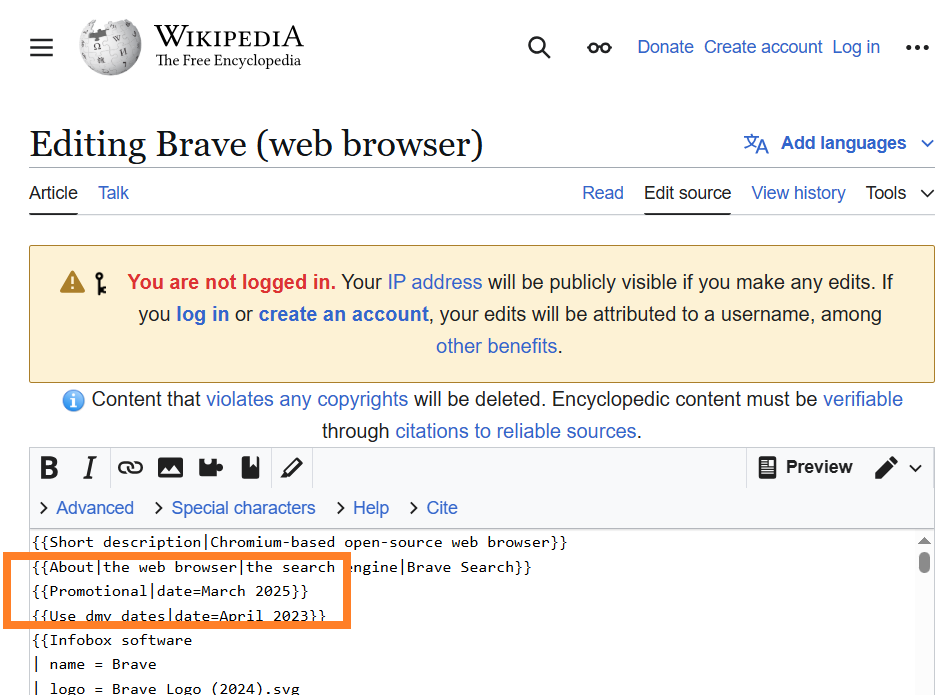
\includegraphics[width=0.6\linewidth]{figures/wp-screenshot-promo-source.png}
        \caption{\url{https://en.wikipedia.org/w/index.php?title=Brave_(web_browser)&action=edit}}
    \end{figure}
\end{frame}

\section{Daten}

\begin{frame}{Daten}
    % Es sollte etwas zur Einleitung der Section gesagt werden
\end{frame}

\subsection{Problemstellung}

\begin{frame}{Problemstellung}
    \begin{block}{Good articles}
        \begin{itemize}
            \item Müssen unter anderem die folgenden Kriterien erfüllen:
            \begin{itemize}
                \item gut geschrieben
                \item korrekte und überprüfbare Informationen
                \item neutral in der Sichtweise
                \item verwenden relevante Bilder mit geeigneten Urheberrechtslizenzen
            \end{itemize}
            \item Nominierung und Vergabe des Status durch die Community (Good article nomination).
            \item 0.59\% aller Wikipedia-Artikel
        \end{itemize}
    \end{block}
\end{frame}

\begin{frame}{Problemstellung}
    \begin{block}{Articles with a promotional tone}
        \begin{itemize}
            \item Artikel, die einer Überarbeitung bedürfen:
            \begin{itemize}
                \item Werbung
                \item Interessenkonflikte
                \item Aus Sicht eines Fans
                \item Pressemitteilungen
                \item Wie ein Lebenslauf
            \end{itemize}
            \item Entsprechende Templates können durch jeden Autoren zum Artikel hinzugefügt oder entfernt werden.
        \end{itemize}
    \end{block}
\end{frame}

\begin{frame}{Problemstellung}
    \begin{block}{Problemstellung}
        \begin{itemize}
            \item Handelt es sich bei einem gegebenen Wikipedia-Artikel um einen guten Artikel, um einen problematischen oder gehört er zu keiner der beiden Klassen?
            \item Falls der Artikel einer Überarbeitung bedarf, was sind die Gründe dafür?
        \end{itemize}
    \end{block}
\end{frame}

\subsection{Datensatz}

\begin{frame}{Datensatz}
    \begin{block}{Kaggle - Wikipedia Promotional Articles}
        \begin{itemize}
            \item Hochgeladen Oktober 2019.
            \item Enthält alle Artikel der englischen Wikipedia, die zum damaligen Zeitpunkt als "good" bzw. "with a promotional tone" markiert waren.
            \item Zwei CSV-Dateien: \texttt{good.csv}, \texttt{promotional.csv}.
            \item \texttt{promotional}-Daten mit jeweils mindestens einem Label versehen: \texttt{advert}, \texttt{coi}, \texttt{fanpov}, \texttt{pr}, \texttt{resume}
        \end{itemize}
    \end{block}
\end{frame}

\begin{frame}{Datensatz}
    \begin{figure}
        \centering
        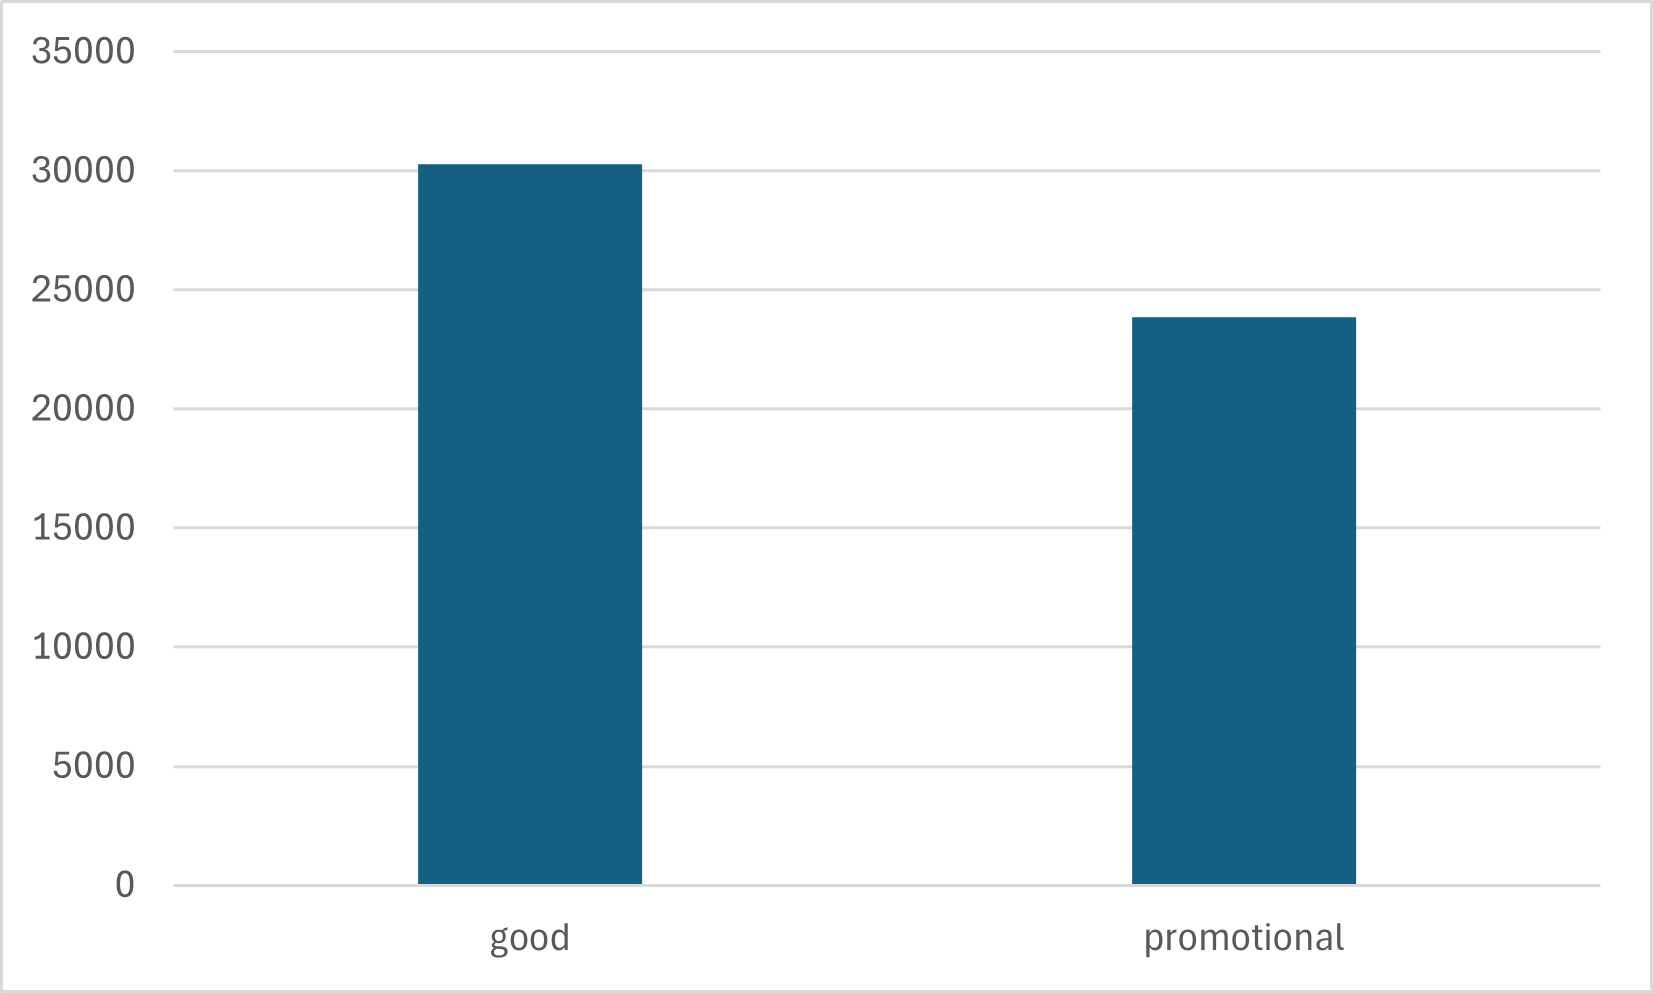
\includegraphics[width=0.6\linewidth]{figures/kaggle-classes.png}
        \caption{Kaggle - Wikipedia Promotional Articles (Classes)}
    \end{figure}
\end{frame}

\begin{frame}{Datensatz}
    \begin{figure}
        \centering
        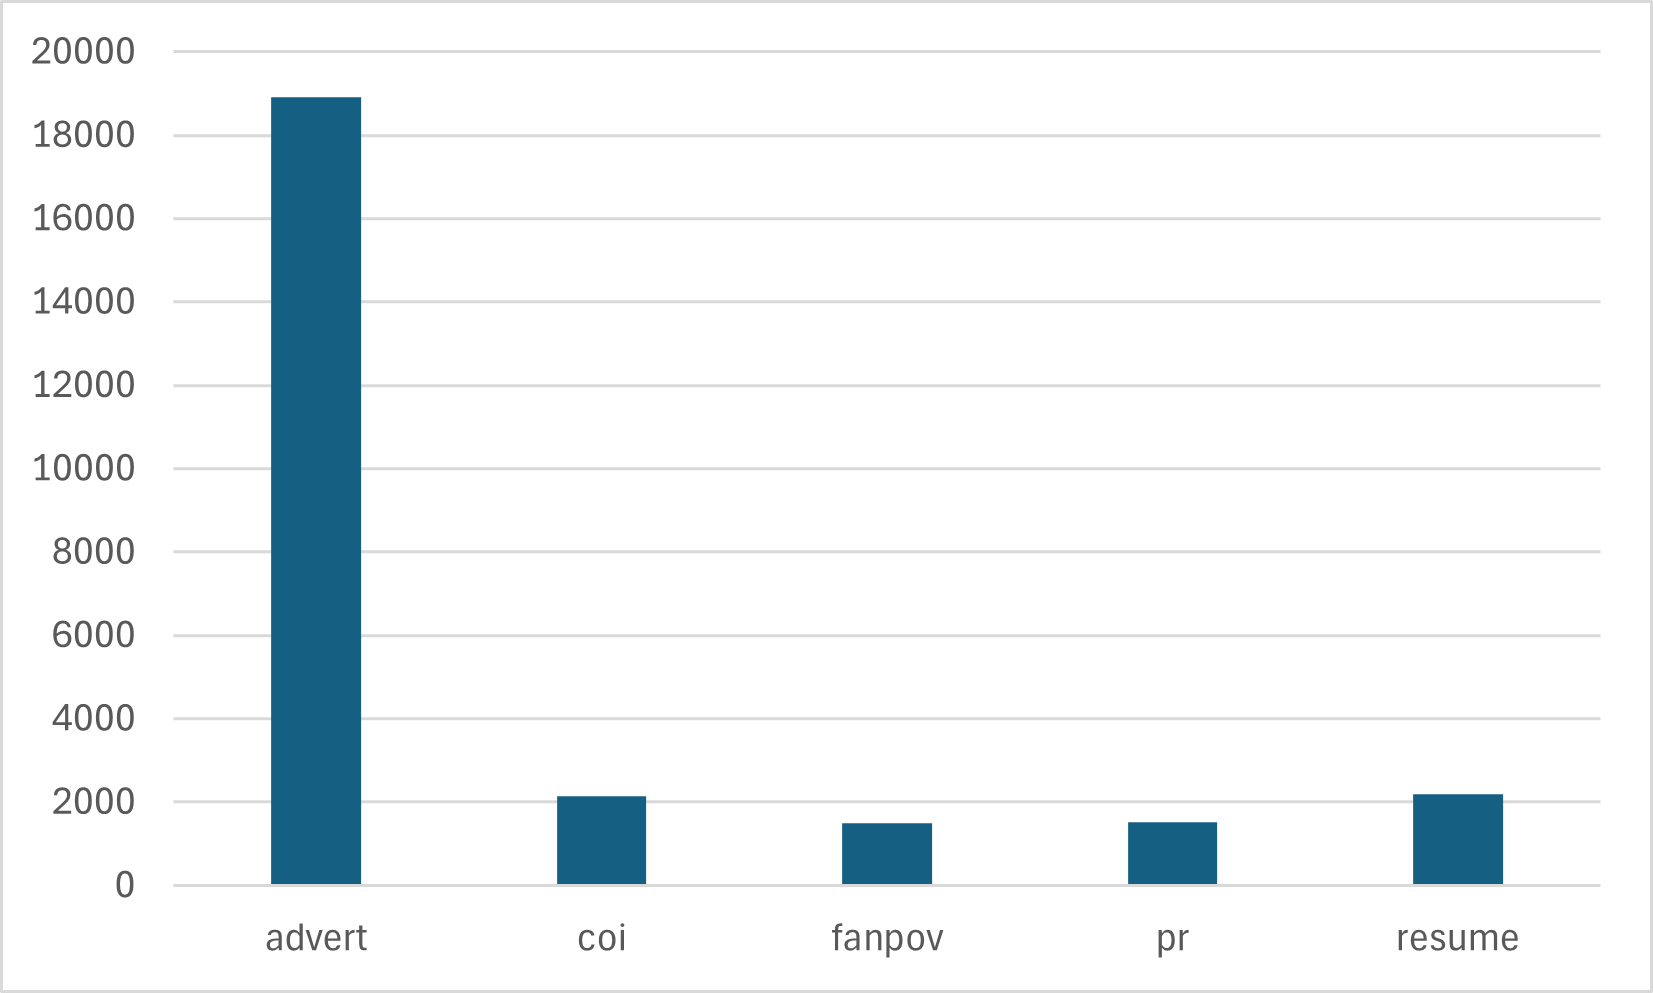
\includegraphics[width=0.6\linewidth]{figures/kaggle-promo-labels.png}
        \caption{Kaggle - Wikipedia Promotional Articles (Labels)}
    \end{figure}
\end{frame}

\subsection{Weitere Daten}

\begin{frame}{Weitere Daten}
    \begin{block}{Einschränkungen des Kaggle-Datensatzes}
        \begin{itemize}
            \item Nicht mehr aktuell: Stand 2019.
            \item Fast 99\% der Artikel sind nicht enthalten, weil sie zu keiner der beiden Klassen gehören.
        \end{itemize}
    \end{block}
\end{frame}

\begin{frame}{Weitere Daten}
    \begin{block}{Wikipedia-Dump}
        \begin{itemize}
            \item Abzüge aller Wikimedia-Datenbanken werden zum Download angeboten.
            \item Aktualisierung zwei Mal monatlich (Angaben beziehen sich auf Dez. 2024).
            \item Englischsprachige Wikipedia ohne Historie ca. 22 GB komprimiert, 97 GB entpackt.
            \item Enthält ca. 24 Mio. Wikipedia-Seiten, darunter ca. 7 Mio. Artikel.
        \end{itemize}
    \end{block}
    \begin{block}{Konvertierung}
        \begin{itemize}
            \item Entpacken und Verarbeiten in Blöcken von je 100 Seiten.
            \item Nicht-Artikel-Seiten erkennen und ausschließen.
            \item Erkennen der Klassen anhand von Templates im Quelltext.
        \end{itemize}
    \end{block}
\end{frame}

\begin{frame}{Weitere Daten}
    \begin{block}{Wikipedia-Dump - Verteilung}
        \begin{itemize}
            \item Klassen der englischsprachigen Artikel:
            \begin{itemize}
                \item good: 46.882
                \item promotional: 32.633
                \item neutral: 6.611.303
            \end{itemize}
            \item Stark unausgeglichen, Reduktion durch Undersampling.
        \end{itemize}
    \end{block}
\end{frame}

\subsection{Vorverarbeitung}

\begin{frame}{Vorverarbeitung}
    \begin{block}{Datensatzvorverarbeitung}
        \begin{itemize}
            \item Extrahieren von Labeln aus Metadaten
            \item Reduzieren auf Artikeltext und Label
            \item Zusammenführen mehrerer Dateien in ein DataFrame
        \end{itemize}
    \end{block}
    \begin{block}{Textvorverarbeitung}
        \begin{itemize}
            \item Entfernen von Sonder- und Interpunktionszeichen
            \item Umwandeln in Kleinbuchstaben
            \item Entfernen von Stoppwörtern
            \item Umwandeln mit Stemming (PorterStemmer)
            \item Zahlen bleiben erhalten
        \end{itemize}
    \end{block}
\end{frame}

% Kandidat für Appendix
\begin{frame}{Vorverarbeitung}
    \begin{exampleblock}{Textvorverarbeitung Artikel 39582}
        \begin{tabularx}{\textwidth}{>{\raggedright\arraybackslash}X >{\raggedright\arraybackslash}X}
            \textbf{Original} & \textbf{Verarbeitete Version}                                                                                                                                                                                                 \\ \hline
            The Human Research Program HRP was created in October 2005 at Johnson Space Center JSC in response to NASA's desire to move human research project management away from headquarters to JSC and to focus its research investment on investigating and mitigating the highest risks to astronaut health and performance in support of exploration missions...
                              &
            human research program hrp creat octob 2005 johnson space center jsc respons nasa desir move human research project manag away headquart jsc focu research invest investig mitig highest risk astronaut health perform support explor mission ... \\
        \end{tabularx}
    \end{exampleblock}
\end{frame}

\begin{frame}{Vorverarbeitung}
    \begin{block}{TF-IDF Vektorisierung}
        \begin{itemize}
            \item Term Frequency-Inverse Document Frequency (TF-IDF) zur Textvektorisierung
            \item Bewertet Wichtigkeit eines Wortes in einem Dokument relativ zum Korpus
            \item Vorteile:
                  \begin{itemize}
                      \item Reduziert Einfluss häufiger, aber uninformativer Wörter
                      \item Hebt diskriminierende Begriffe hervor
                      \item Erzeugt spärliche Merkmalsvektormatrizen
                  \end{itemize}
            \item Parameter:
                  \begin{itemize}
                      \item \texttt{ngram\_range: [1, 1]} - Nur Einzelwörter werden betrachtet
                            % Mehrwort-Ausdrücke (n-grams) werden nicht berücksichtigt
                      \item \texttt{max\_df: 0.9} - Ignoriert Korpus-spezifische Stopwörter ($>90\%$)
                            % Entfernt häufige Wörter, die in fast allen Dokumenten vorkommen
                      \item \texttt{min\_df: 0.001} - Filtert Rauschen und Rechtschreibfehler ($<0.1\%$)
                            % Entfernt sehr seltene Wörter, reduziert Vokabulargröße und Overfit-Risiko
                      \item \texttt{max\_features: 10\_000} - Beschränkt die Vokabulargröße auf 10.000
                            % Verbessert Laufzeiteffizienz und verringert Overfit-Risiko
                      \item \texttt{sublinear\_tf: true} - Logarithmische TF-Skalierung für lange Dokumente
                            % Reduziert Verzerrungen durch mehrfach vorkommende Wörter in einem Dokument
                  \end{itemize}
        \end{itemize}
    \end{block}
\end{frame}

\begin{frame}{Easy Data Augmentation (EDA)}
    \begin{block}{Ziel und Methode}
        \begin{itemize}
            \item Idee: Die Anwendung von Easy Data Augmentation (EDA), um durch augmentierte Daten die Anzahl der unterrepräsentierten Labels zu vergrößern.
        \end{itemize}
    \end{block}

    \begin{block}{Umsetzung}
        \begin{itemize}
            \item Es wurden neue Texte aus den Originaltexten erstellt indem Synonyme hinzugefügt, zufällig Wortreihenfolgen getauscht und zufällig Wörter eingefügt bzw. gelöscht worden sind.
        \end{itemize}
    \end{block}

    \begin{alertblock}{Ergebnisse}
        \begin{itemize}
            \item Auf dem augmentierten Datensatz trainierte Modelle verbesserten sich signifikant, wenn auf den augmentierten Daten getestet worden ist. Das augmentierte Modell schnitt aber deutlich schlechter ab, wenn auf dem Originalsatz getestet worden ist. Damit zeigt sich der Verdacht von Overfitting. $\to$ \textbf{Ansatz verworfen}.
        \end{itemize}
    \end{alertblock}
\end{frame}

\section{Ansätze}

\begin{frame}{Ansätze}
    \begin{block}{Klassische Verfahren}
        \begin{itemize}
            \item Logistische Regression
            \item Bayes-Klassifikator
            \item Support Vector Machine
        \end{itemize}
    \end{block}
    \begin{block}{Deep Learning}
        \begin{itemize}
            \item \yellowhighlight{CNN}
            \item \yellowhighlight{5. Ansatz}
        \end{itemize}
    \end{block}
\end{frame}

\subsection{Klassische Verfahren}

\begin{frame}{Klassische Verfahren}
    \begin{block}{Logistische Regression}
        \begin{itemize}
            \item Diskriminativer Klassifikator, der Entscheidungsgrenzen direkt modelliert
            \item Schätzt die Wahrscheinlichkeiten von Klassen basierend auf einer linearen Entscheidungsfunktion
            \item Geeignet für Textklassifikation mit hochdimensionalen Feature-Vektoren
            \item Vorteile:
                  \begin{itemize}
                      \item Lineare Zeitkomplexität O(nd) % SB: Sicher? Logreg hatte mit Abstand das längste Training der drei klassischen Modelle
                      \item Einfach Implementation
                      \item Schnell in der Berechnung.
                  \end{itemize}
            \item Parameter:
                  \begin{itemize}
                      \item \texttt{Regularisierung}: L1-Regularisierung
                      \item \texttt{OneVsRestClassifier}: Für die Klassifizierung der Multilabeldaten
                  \end{itemize}
        \end{itemize}
    \end{block}
\end{frame}

\begin{frame}{Klassische Verfahren}
    \begin{block}{Multinomialer Naive Bayes-Klassifikator}
        \begin{itemize}
            \item Probabilistischer Klassifikator, der auf Bayes'schem Theorem basiert
            \item Nimmt bedingte Unabhängigkeit zwischen Features an (naive Annahme)
            \item Geeignet für Textklassifikation mit Wortvorkommen als Features
            \item Vorteile:
                  \begin{itemize}
                      \item Lineare Zeitkomplexität O(nd) % n = Anzahl der Features, d = Anzahl der Klassen
                            % Mit Abstand der schnelleste Klassifikator gerade beim gesampelten Wikipedia-Dump
                            % Training auf den samples war nach Sekunden abgeschlossen
                      \item Robust bei hoher Dimensionalität
                            % Die vektorisierten Features sind hochdimensional
                            % (Definition hochdimensional?)
                      \item Native Unterstützung für spärliche Matrizen
                            % die vektorisierten Features sind spärliche Matrizen
                  \end{itemize}
            \item Parameter:
                  \begin{itemize}
                      \item \texttt{alpha}: Laplace-Glättung
                            % Wird verwendet, um Überanpassung zu vermeiden, indem Null-Wahrscheinlichkeiten durch eine kleine positive Konstante ersetzt werden
                      \item \texttt{fit\_prior}: Lernen der Klassenpriors
                            % Wird verwendet, um die Klassenverteilung aus den Trainingsdaten zu schätzen bevor man irgendwelche Features sieht. Wenn False wird gleiche Klassenwahrscheinlichkeit angenommen
                  \end{itemize}
        \end{itemize}
    \end{block}
\end{frame}

\begin{frame}{Klassische Verfahren}
    \begin{block}{Support Vector Machine (SVM)}
        \begin{itemize}
            \item Nutzt den Konzept des maximalen Margins, um eine robuste Trennlinie zu finden
            \item Kann mit Kernelfunktionen erweitert werden, um nicht-lineare Trennungen zu ermöglichen
            \item Geeignet für hochdimensionale Datenräume, insbesondere für Textklassifikation
            \item Parameter:
                  \begin{itemize}
                      \item \texttt{C}: Regularisierungsparameter zur Steuerung des Trade-offs zwischen Maximierung des Margins und Minimierung von Fehlklassifikationen
                      \item \texttt{kernel}: Auswahl der Kernel-Funktion (z.B. linear, RBF, polynomial)
                      \item Kernel-spezifische Parameter
                  \end{itemize}
        \end{itemize}
    \end{block}
\end{frame}


\begin{frame}
    \begin{block}{Gemeinsamkeiten}
        \begin{itemize}
            \item GridSearchCV von sklearn wurde für eine Hyperparameter-Optimierung nach Recall verwendet
            \item OneVsRestClassifier von sklearn wurde für Multilabel-Klassifikation verwendet
        \end{itemize}
    \end{block}
\end{frame}

\subsection{Deep Learning}

\begin{frame}{Deep Learning}
    CNN
\end{frame}

\begin{frame}{Deep Learning}
    \begin{block}{5. Ansatz}
        Probleme: Schlechte Multilabelklassifizierung der ersten vier Ansätze. \\
        Analyse: Unterscheidung der Promotional aufgrund von Thema: \\
        Ziel:
        Einbezug von Kontext/Bedeutung \\
        Ideen:
        \begin{itemize}
            \item Vorverarbeitungsmethode erstellen
            \item Transformerarchitektur verwenden
        \end{itemize}
    \end{block}
\end{frame}

\begin{frame}{Deep Learning}
    \begin{block}{Transformerarchitektur}
        Modellwahl: DistilBERT \\
        Vorteile: Besondere Vorteile von BERT in der Erkennung von Kontext \\
        Architektur:
        \begin{itemize}
            \item Darstellung: DistilBERT Tokenizer
            \item Attention: Scaled Dot Product Attention (SDPA)
            \item Aktivierungsfunktion: $GeLu(x) \approx {0.5 \cdot x \cdot (1+ tanh({\frac{x}{\sqrt{2}}}))} $
        \end{itemize}
    \end{block}
\end{frame}

\section{Zusammenfassung}

\begin{frame}{Zusammenfassung}
    \begin{block}{Zusammenfassung}
        Errungenschaften:
        \begin{itemize}
            \item Daten analysiert
            \item Datensatz mit Wikipedia Dump erweitert
            \item Problemstellung erfasst
            \item Datensatz für Mashine Learning Verfahren vorbereitet.
            \item Drei Klassische Modelle implementiert
            \item Zwei Neuronale Methode implementiert
            \item Ergebnisse Evaluiert
        \end{itemize}
        Ergebnisse:
        \begin{itemize}
            \item Datensatz aus Wikipedia Dump erstellt
            \item Pipeline zur Klassifizierung von Wikipediaartikeln implementiert
        \end{itemize}
    \end{block}
\end{frame}

\begin{frame}{Zusammenfassung}
    \begin{block}{Zusammenfassung}
        Misserfolge
        \begin{itemize}
            \item Datenaugmentierung
            \item Entwicklung von Vorverarbeitung zur Erkennung von Kontext
        \end{itemize}
        Erweiterungsmöglichkeiten:
        \begin{itemize}
            \item Weitere klassische und neuronalen Ansätze implementieren und evaluieren
            \item Ganzen Wikipedia Dump verwenden
            \item Verwendung von SetFit
            \item Verwendung weiterer Modelle des Maschinellen Lernens
        \end{itemize}
    \end{block}
\end{frame}

\appendix
\section{Appendix}

\begin{frame}{Ergebnisse Datenaugmentierung}
    Beispielfolie für Appendix
\end{frame}


\end{document}
